\chapter{Lösungsdesign}

Das Lösungsdesign beinhaltet die Grundlagen für die erfolgreiche Umsetzung des Prototyps. Vor der eigentlichen Implementation wird das Vorhaben auf konzeptioneller Ebene genauer betrachtet. Die Definition der Schnittstellen, besonders die Verminderung der Kopplung zwischen der Visualisierung und dem \gls{ikc-core}, ist hier ein wichtiger Punkt.


%Dieses Kapitel beinhaltet die definierten Schnittstellen sowohl die Auswahl des Frameworks für die Darstellung. Ein besonderes Augenmerk wird auf die Interaktion zwischen der Visualisierung und dem \textit{ikc-core} gelegt, besonders auf die Verminderung der Kopplung zwischen den beiden Komponenten. 

\section{User Interface Design}

Nachfolgend werden wichtige Punkte zum Umgang mit dem \gls{Netzwerk} und zur Integration der Visualisierung aufzeigt und weitergehende Überlegungen dazu dargelegt.

\subsection{Umgang mit dem Netzwerk}

Die Benutzeroberfläche orientiert sich hauptsächlich am \gls{Netzwerk}, bestehend aus \gls{Node}[s] und \gls{Link}[s]. Diese besitzen eine Beschriftung in Form des Titels oder in Form des entsprechenden \gls{Tags} (\autoref{fig:nodes-links}). Die Beschriftung kann zugunsten der Übersichtlichkeit gegebenenfalls ausgeblendet werden.

Wo immer möglich soll die Interaktion nicht über eine entfernte Schaltfläche, sondern direkt am jeweiligen Element in der Visualisierung geschehen. Ein mögliches Beispiel hierfür zeigt \autoref{fig:node-menu}. Am Knoten, wo eine Aktion vorgenommen werden soll, kann mittels eines Klicks (oder Ähnlichem) ein Kontextmenü geöffnet werden. Dieses ermöglicht der Situation entsprechende, weiterführende Funktionalitäten. Entsprechende Möglichkeiten sind auch beim Umgang mit Kanten vorstellbar.

\begin{figure}[htbp]
\centering
 \begin{subfigure}[b]{0.35\textwidth}
        \centering
        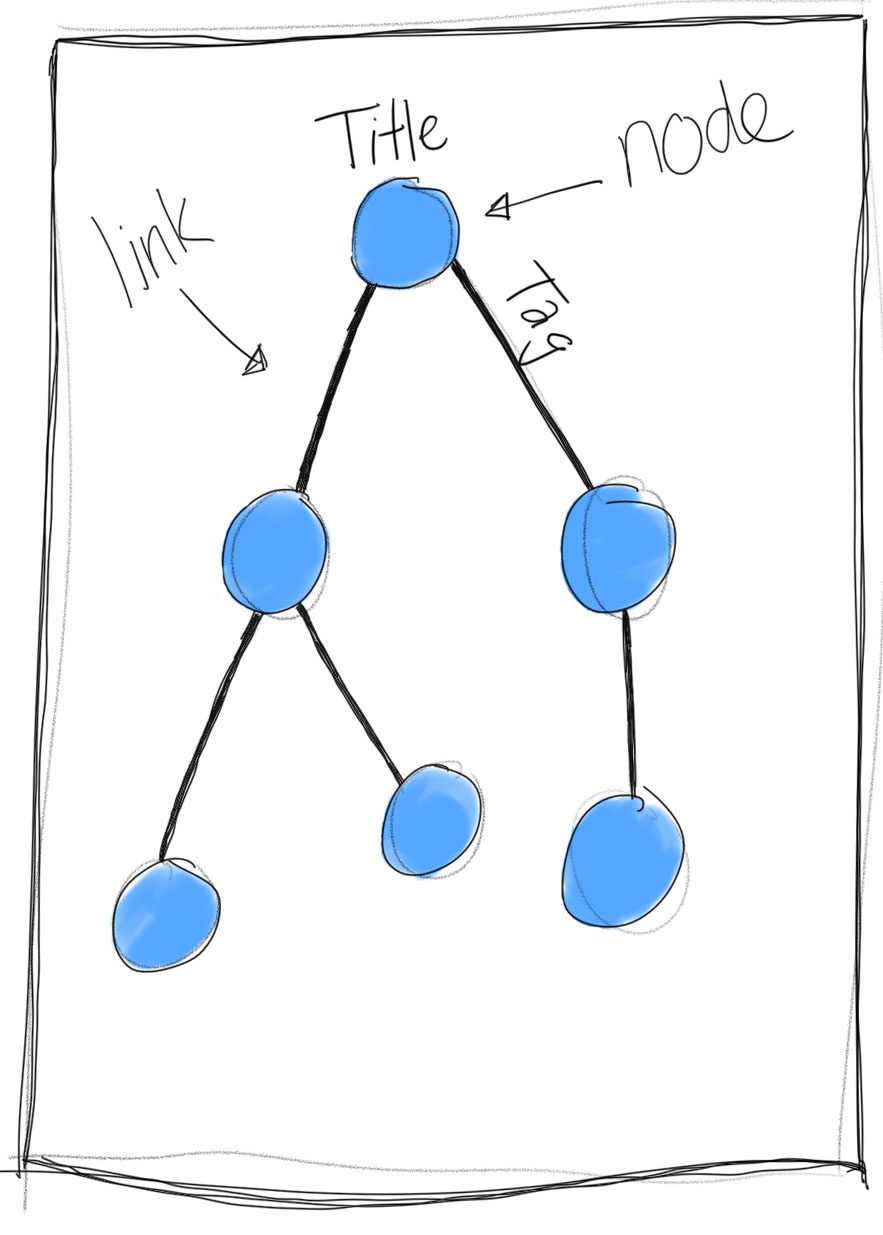
\includegraphics[width=0.9\linewidth]{skizze-nodes-links}
        \caption{Nodes und Links}
        \label{fig:nodes-links}
    \end{subfigure}
 \begin{subfigure}[b]{0.35\textwidth}
        \centering
        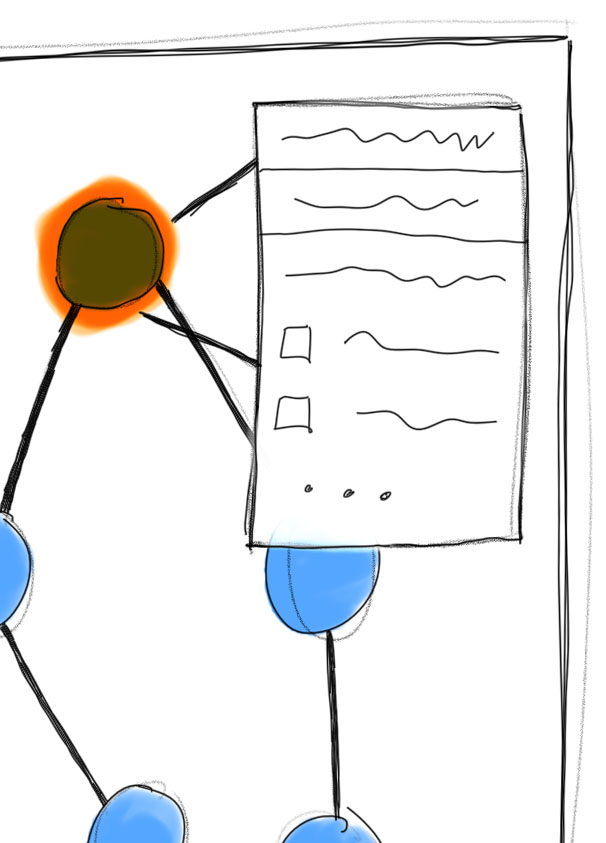
\includegraphics[width=0.9\linewidth]{skizze-contextmenu}
        \caption{Node-Menü}
        \label{fig:node-menu}
    \end{subfigure}
    \caption{Skizzen: Benutzeroberfläche}
\end{figure}


\subsection{Komponenten der Benutzeroberfläche}\label{komponenten}

Die Visualisierung verwendet Komponenten, welche Funktionen für den Benutzer zusammenfassen oder als Container für weitere Elemente dienen können. In der späteren Implementation werden diese komplett oder teilweise direkt mit einer \hyperref[react]{\textit{React}}-Komponente realisiert.

%Für die Visualisierung verwenden wir verschieden Element, in welchen Funktionen für den Benutzer zusammengefasst werden oder auch als Container für weiter Inhalte dienen. Diese werden dann in der Implementation durch eine \gls{React} Komponente oder einen Teil einer repräsentiert. 

\subsubsection{GraphScreen}
Der \textit{GraphScreen} (\autoref{fig:graph-screen-draw}) beinhaltet alle wesentlichen Elemente der Visualisierung. Dazu gehört in erster Linie das \gls{Netzwerk}, in welchem die \gls{Node}[s] und \gls{Link}[s] dargestellt werden. Weiter ist eine Navigationsleiste (\textit{Toolbar}) enthalten, in welcher wichtige Funktionen zur Verfügung gestellt werden. 

\begin{figure}[htbp]
    \centering
     \begin{subfigure}[b]{0.4\textwidth}
    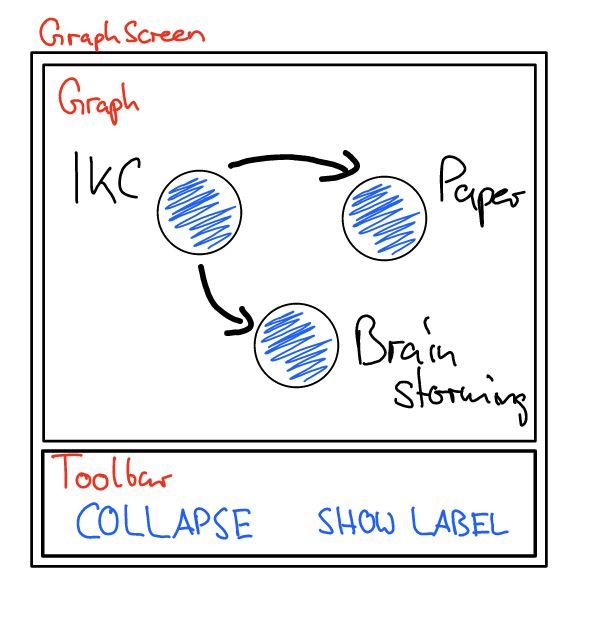
\includegraphics[width=1\linewidth]{GraphScreen}
    \caption{GraphScreen}
    \label{fig:graph-screen-draw}
    \end{subfigure}
    \begin{subfigure}[b]{0.5\textwidth}
    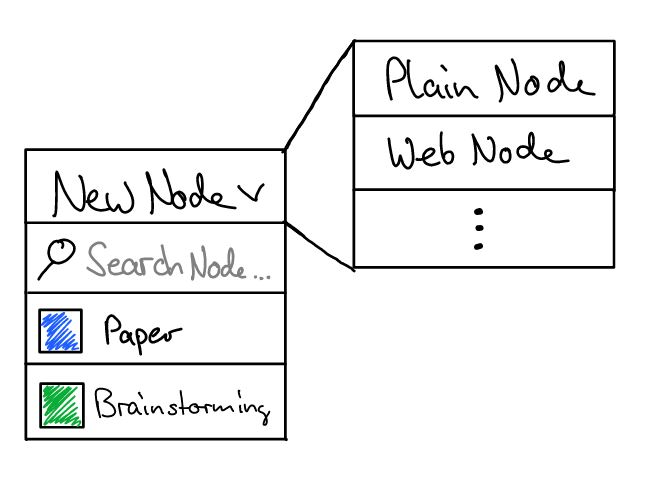
\includegraphics[width=1\linewidth]{CoreContextMenu}
    \caption{CoreContextMenu}
    \label{fig:core-context-menu}
    \end{subfigure}
    \caption{Skizzen: Benutzeroberfläche}
\end{figure}

\subsubsection{CoreContextMenu}
Das über einen \textit{Rechtsklick} (Desktop) bzw. \textit{Tap} (Mobile) zu öffnende \textit{CoreContextMenu} macht für den gegebenen Kontext weitere Funktionen abrufbar (\autoref{fig:core-context-menu}). Dabei geht es in erster Linie darum in der Visualisierung neue \gls{Node}[s] darzustellen. Einerseits können neue \gls{Node}[s] erstellt, andererseits über die Suchfunktion (auch in der Datenbasis bestehende) gefunden und verwendet werden. Der neu hinzugefügtn Knotenbefindet sich automatisch an jener Position, wo das Menü geöffnet wurde.

% So können verschiedenen Dialoge aufgerufen werden um unterschiedliche \gls{Node}[s] zu erstellen und in der Sicht darzustellen oder über ein Such Feld können bestehende Node der Sicht hinzugefügt werden. Der resultierende neue Node wird dabei an derselben Stelle dargestellt wo das Menu geöffnet wurde. Das Öffnen des Menüs erfolgt dabei durch einen \textit{Rechtsklick} (Desktop) oder \textit{Tap} (Mobile). 


\subsubsection{NodeContextMenu}
Aktionen, welche auf einen spezifischen \gls{Node} angewendet werden, sind im \textit{NodeContextMenu} zusammengefasst (\autoref{fig:node-context-menu}). Dazu zählen Aktionen, mit welchen der entsprechende \gls{Node} oder dessen \gls{Link}[s] bearbeitet werden können. Auch dieses Menü öffnet sich durch einen \textit{Rechtsklick} (Desktop) oder \textit{Tap} (Mobile). 


\begin{figure}[htbp]
\centering
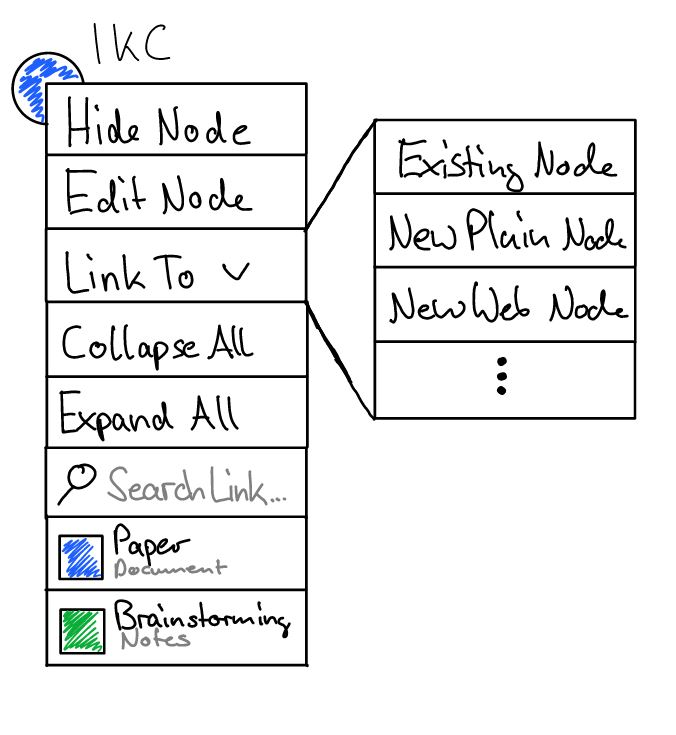
\includegraphics[width=0.5\textwidth]{NodeContextMenu}
\caption{Skizze: NodeContextMenu}
\label{fig:node-context-menu}
\end{figure}

\subsection{Aktionen}
\label{subsec:aktionen}
In einem Menu, der Toolbar oder durch ein \gls{Drag'n'Drop} können verschiedene Funktionen auf einzelne \gls{Node}[s], \gls{Link}[s] oder das gesamte \gls{Netzwerk} angewendet werden. Dazu gehören:

    \begin{longtable}{|P{2cm}|P{5cm}||p{0.3cm}|p{0.3cm}|p{0.3cm}|p{0.3cm}|p{0.3cm}|p{0.3cm}|}
  \hline
    Aktion & Beschreibung & \rotatebox[origin=c]{90}{CoreContextMenu}& \rotatebox[origin=c]{90}{NodeContextMenu}& \rotatebox[origin=c]{90}{Toolbar}& \rotatebox[origin=c]{90}{Drag'n'Drop}& \rotatebox[origin=c]{90}{Click}& \rotatebox[origin=c]{90}{Tab}\\\hline
    \textit{Edit Node} & Einen \gls{Node} bearbeiten. &&x&&&x& \\\hline
    \textit{Add Node} & Einen existierenden \gls{Node} aus der Datenbasis der Visualisierung hinzufügen. Dabei werden alle \gls{Link}[s] und deren Ziel-Nodes ebenfalls dargestellt. &x&&&x&& \\\hline
    \textit{Hide Node} & Einen \gls{Node} mit seinen \gls{Link}[s] aus der Sicht entfernen (nicht aber aus der Datenbasis). &&x&&&& \\\hline
    \textit{Delete Node} & Das Löschen eines \gls{Node}[s] aus der Sicht und der Datenbasis. Dies ist nur möglich durch die Bearbeitung des \gls{Node}[s] in der Detailansicht. &&&&&& \\\hline
    \textit{Delete Link} & Das Löschen eines \gls{Link}[s] aus der Sicht und der Datenbasis. Dies ist nur möglich durch die Bearbeitung des \gls{Node}[s] in der Detailansicht. &&&&&& \\\hline
    \textit{New Node} &  Einen neuen \gls{Node} erstellen. &x&&&&& \\\hline
    \textit{New Link} & Einen neuen \gls{Link} zwischen zwei \gls{Node}[s] erstellen. Hierzu wird ein \gls{Node} über einen anderen gezogen und losgelassen. (\autoref{fig:add-link}). &&&&x&& \\\hline
    \textit{Link To New Node} & Neuen \gls{Node} erstellen und anschliessend mit einem anderen \gls{Node} durch einen \gls{Link} verbinden. &&x&&&& \\\hline
    \textit{Link To Existing Node} & \gls{Link} zu einem existierenden \gls{Node} in der Datenbasis erstellen. &&x&&x&& \\\hline
    \textit{Collapse All} & Alle ausgehenden \gls{Link}[s] des entsprechenden \gls{Node}[s] werden zusammen mit ihren Ziel-Nodes ausgeblendet. Falls der Ziel-Node noch über andere \gls{Link}[s] verfügt, wird nur der \gls{Link} zwischen dem \gls{Node} und dem Ziel-Node ausgeblendet (\autoref{fig:collapse-all}). &&x&&&& \\\hline
    \textit{Select Link} & \gls{Link}[s] auswählen, um eine weitere Aktion auf alle anwenden zu können. &&&&&x&x \\\hline
    \textit{Collapse Links} & Ausgewählte \gls{Link}[s] werden zusammen mit ihren Ziel-Nodes ausgeblendet. Falls der Ziel-Node noch über andere \gls{Link}[s] verfügt, wird nur der \gls{Link} zwischen dem \gls{Node} und dem Ziel-Node ausgeblendet (\autoref{fig:collapse-link}). &&&x&&& \\\hline
    \textit{Expand All} & Alle ausgehenden \gls{Link}[s] eines entsprechenden \gls{Node}[s] werden zusammen mit deren Ziel-Nodes eingeblendet (\autoref{fig:expand-all}). &&x&&&& \\\hline
    \textit{Expand Link} & Einen ausgehenden \gls{Link} eines \gls{Node} darstellen. &&x&&&& \\\hline
    \textit{Show/Hide Labels} & Beschreibungen der \gls{Link}[s] darstellen oder ausblenden. &&&x&&& \\\hline
    \textit{Update Position} & Ein \gls{Node} kann neu positioniert werden. &&&&x&& \\\hline
    \caption{Funktionen}
  \label{tab:funktionen}
\end{longtable}


% \begin{figure}
%    \centering
%     \begin{subfigure}{0.4\textwidth}
%    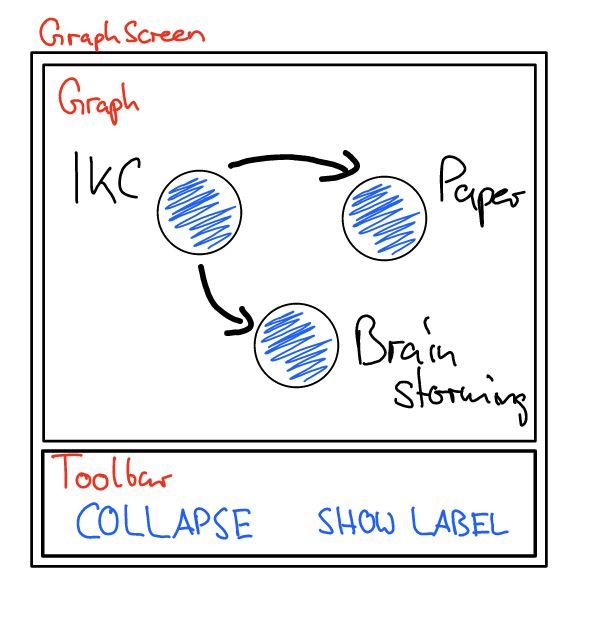
\includegraphics[width=0.9\linewidth]{GraphScreen}
%    \caption{GraphScreen}
%    \label{fig:graph-screen-draw}
%    \end{subfigure}
%    \begin{subfigure}{0.5\textwidth}
%    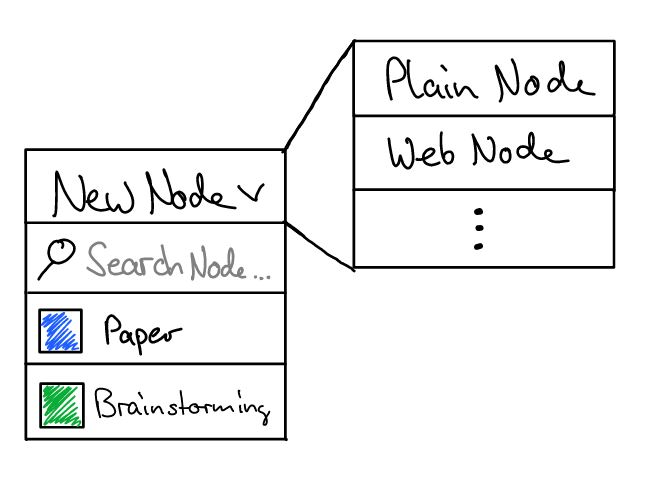
\includegraphics[width=0.9\linewidth]{CoreContextMenu}
%    \caption{CoreContextMenu}
%    \label{fig:core-context-menu}
%    \end{subfigure}
%    \caption{Skizzen Benutzeroberfläche}
%\end{figure}

\begin{figure}[htbp]
\centering
    \begin{subfigure}[b]{0.5\textwidth}
    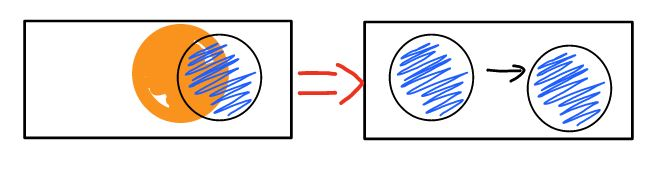
\includegraphics[width=1\linewidth]{AddLink}
    \caption{New Link}
    \label{fig:add-link}
    \end{subfigure}
    \begin{subfigure}[b]{0.4\textwidth}
    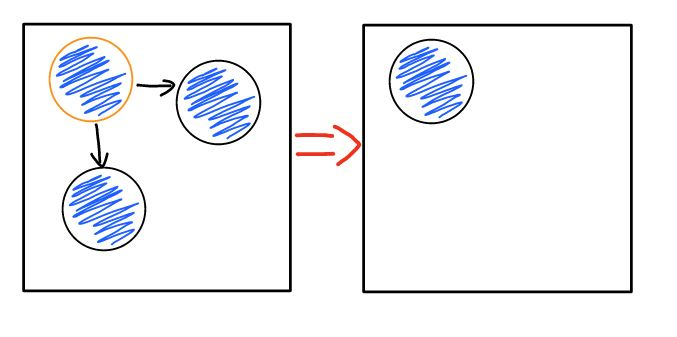
\includegraphics[width=1\linewidth]{CollapseAll}
    \caption{Collapse All}
    \label{fig:collapse-all}
    \end{subfigure}
    \caption{Skizzen: Aktionen}
\end{figure}

\begin{figure}[htbp]
\centering
    \begin{subfigure}[b]{0.4\textwidth}
    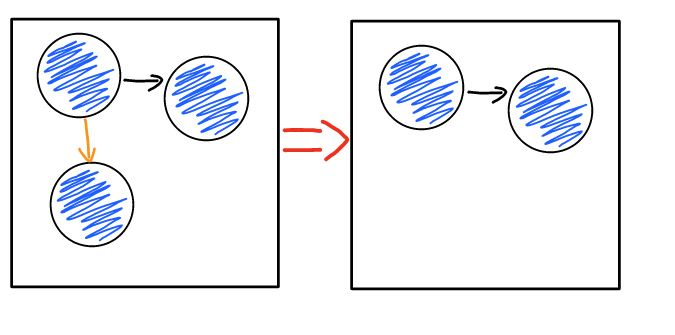
\includegraphics[width=1\linewidth]{CollapseLink}
    \caption{Collapse Link}
    \label{fig:collapse-link}
    \end{subfigure}
    \begin{subfigure}[b]{0.5\textwidth}
    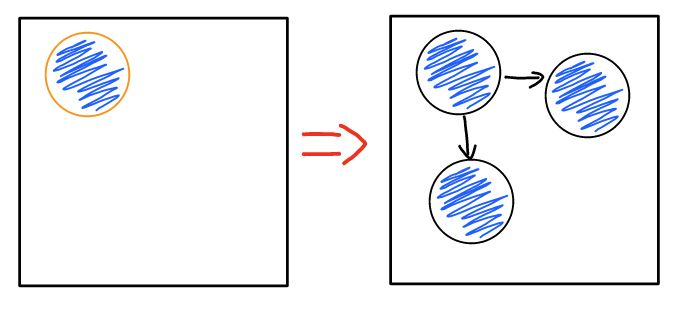
\includegraphics[width=1\linewidth]{ExpandAll}
    \caption{Expand All}
    \label{fig:expand-all}
    \end{subfigure}
    \caption{Skizzen: Aktionen}
\end{figure}


\subsection{Integration}

Aus den Anforderungen geht die Interaktion mit dem \gls{ikc-core} als weiterer wichtiger Punkt hervor. Von besonderer Bedeutung ist hier die Bedienung mittels \gls{Drag'n'Drop}. Wie in \autoref{fig:grenze-core-visual} sichtbar, muss dabei die Grenze zwischen \gls{ikc-core} und der Visualisierung (grüne Linie) überwunden werden. Mittels \gls{Drag'n'Drop} kann also beispielweise ein \gls{Node} aus der \gls{ikc-core}-Komponente (orange) in die Visualisierung positioniert werden. Dort kann dieser weiter mit dem bestehenden \gls{Netzwerk} verknüpft oder als eigenständiger neuer Knoten dargestellt werden.

\begin{figure}[htbp]
\centering
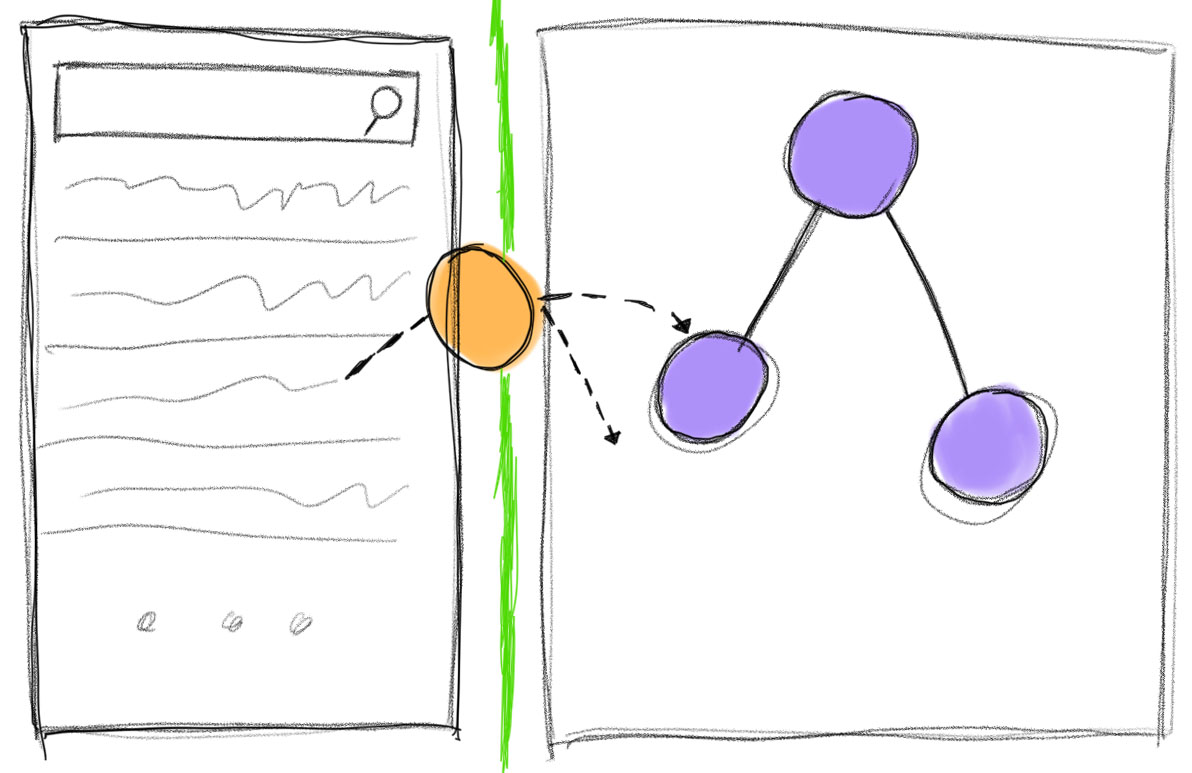
\includegraphics[width=0.5\textwidth]{ikc-core-visual}
\caption{Grenze \gls{ikc-core} - visual}
\label{fig:grenze-core-visual}
\end{figure}

Wo immer möglich, sollen bestehende Komponenten wiederverwendet werden. Dies bietet sich nicht nur bei \autoref{fig:node-menu} in Form eines Kontextmenüs, sondern auch für die Suchfunktion und die Detailansicht an. Für die Desktop-Ansicht wird die Visualisierung mittig in einer dreispaltigen Anordnung in den \textit{ikc-core} eingebettet (\autoref{fig:3-column}). Auf der linken Seite befindet sich die Suche. Auf der rechten Seite die Detailansicht für den in der Visualisierung ausgewählten \gls{Node}. Dort sind auch weitere Optionen in Form von Menüpunkten verfügbar, beispielsweise sind die ausgehenden \gls{Link}[s] erreichbar. Zu\-sätz\-lich gibt es eine übergeordnete Navigationsleiste, wo wichtige Funktion direkt abrufbar sind.

Bei der Version für Tablets und Smartphones sind, je nach verfügbarer Breite, nur eine oder zwei Spalten sichtbar.

\begin{figure}[htbp]
\centering
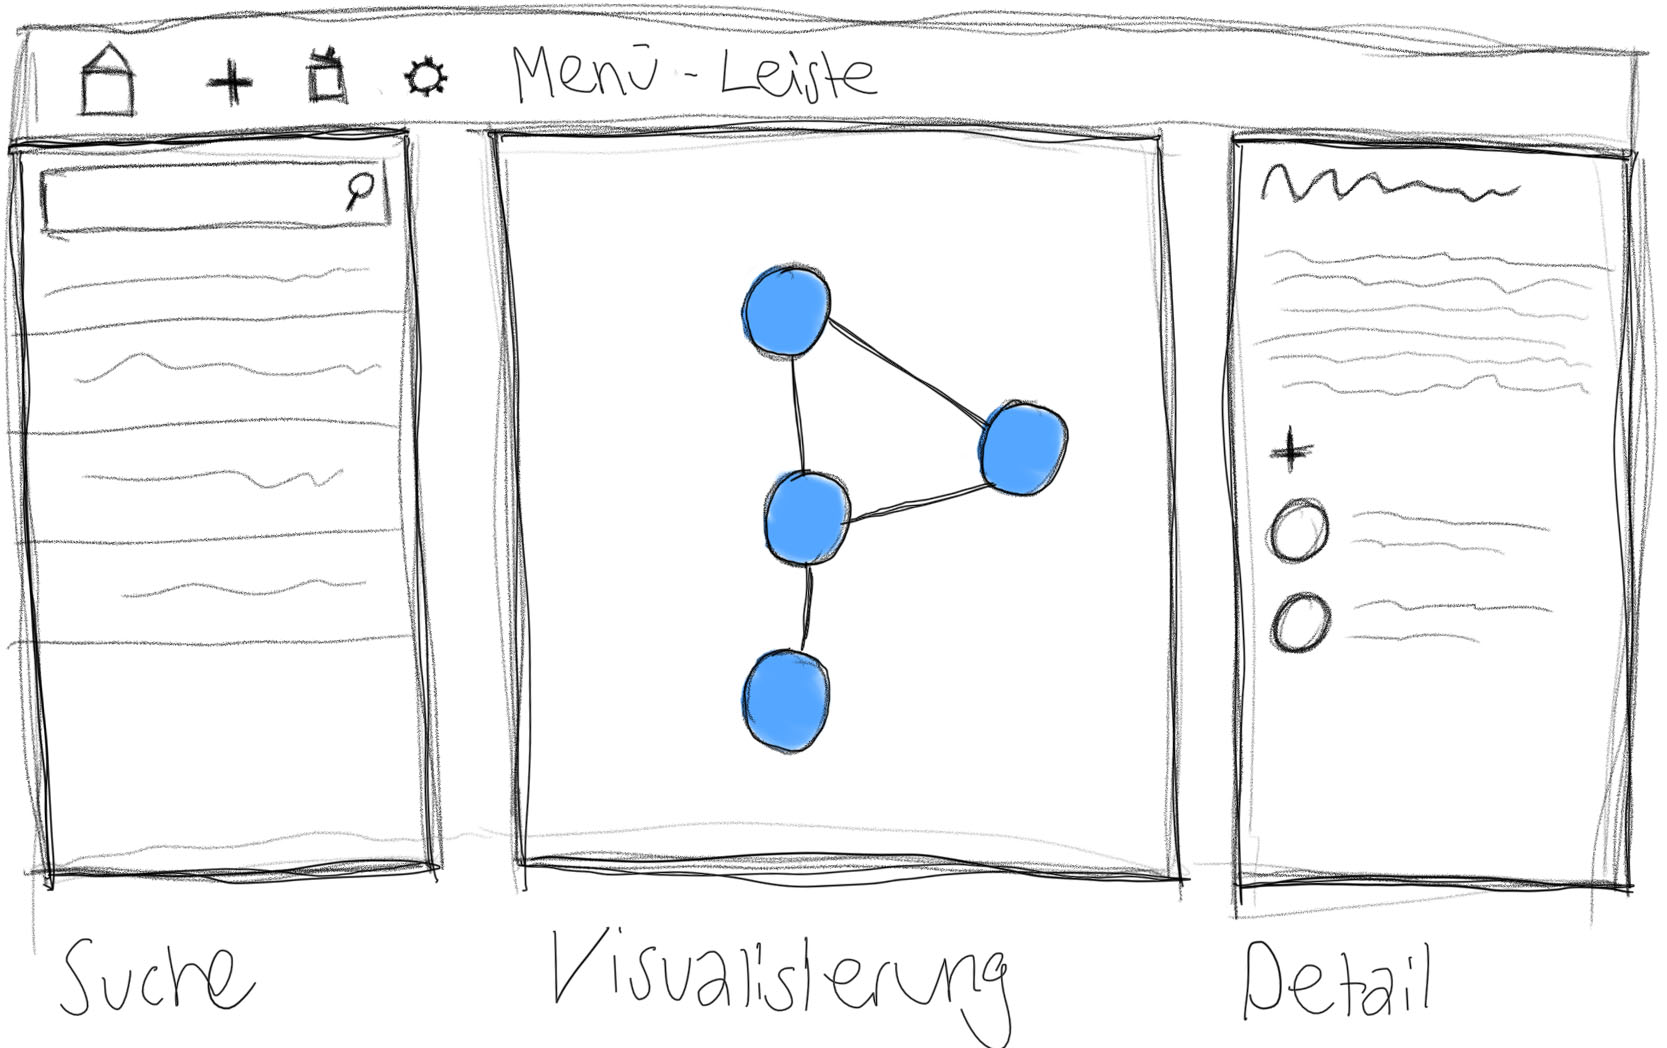
\includegraphics[width=0.8\textwidth]{integration-3-column}
\caption{3-spaltige Oberfläche}
\label{fig:3-column}
\end{figure}

\section{Technische Ausgangslage}
Der \gls{ikc-core} funktioniert momentan mit einer rudimentären Benutzeroberfläche. Die Applikationslogik und der Umgang mit der Datenbasis existieren somit bereits. Wie auf dem Komponentendiagramm (\autoref{fig:komponentendiagramm}) ersichtlich, nutzt der \gls{ikc-core} die Visualisierung (\textit{graph-visualization}). Jedoch müssen dazu verschiedene Schnittstellen der Visualisierung implementiert werden. Diese werden von der Visualisierung genutzt, um Operationen an den \gls{ikc-core} zu delegieren. Dies kann als Nutzungsvertrag zwischen der Visualisierung und der Komponente, welche sie verwendet, verstanden werden. Beispielsweise interessiert es die Visualisierung wenig, wie und wo ein \gls{Node} gespeichert wird. Es wird nur die jeweilige Methode ausgeführt, alles andere geschieht ausserhalb der Vi\-su\-ali\-si\-erung. Mehr Details dazu sind im \autoref{sec:architektur} zu finden.

\begin{figure}[htbp]
\centering
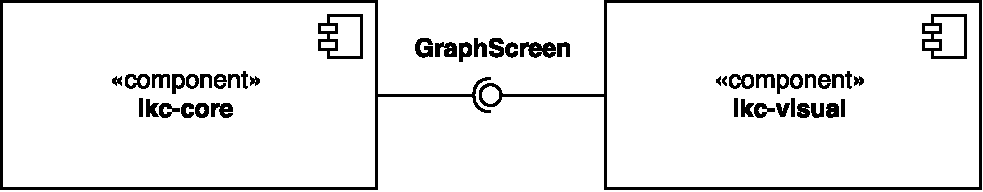
\includegraphics[width=0.6\textwidth]{components}
\caption{Komponentendiagramm}
\label{fig:komponentendiagramm}
\end{figure}

\section{Architektur}
\label{sec:architektur}

Das Klassendiagramm (\autoref{fig:klassendiagramm}) gewährt einen detaillierten Überblick über die Architektur der Visualisierung. Es zeigt die Schnittstellen zum \gls{ikc-core} und die wichtigsten Komponenten auf. Die \hyperref[react]{\textit{React}}-Klasse \textit{GraphScreen} repräsentiert das gesamte Packet ausserhalb der Visualisierung. Sie hält alle internen Klassen, Interfaces und Komponenten zusammen und stellt sicher, dass Informationen zum richtigen Zeitpunkt bei der richtigen Klasse platziert werden. \textit{Graph} als zweite grosse \hyperref[react]{\textit{React}}-Klasse kapselt das \gls{Framework} \textit{cytoscape} und stellt die Interaktion mit der Visualisierung sicher. Die weiteren Schnittstellen, Klassen und ihre Implementationen werden im \autoref{schnittstellen}, \autoref{model} und \autoref{implementation} genauer ausgeführt.

\begin{landscape}
\begin{figure}[htbp]
\centering
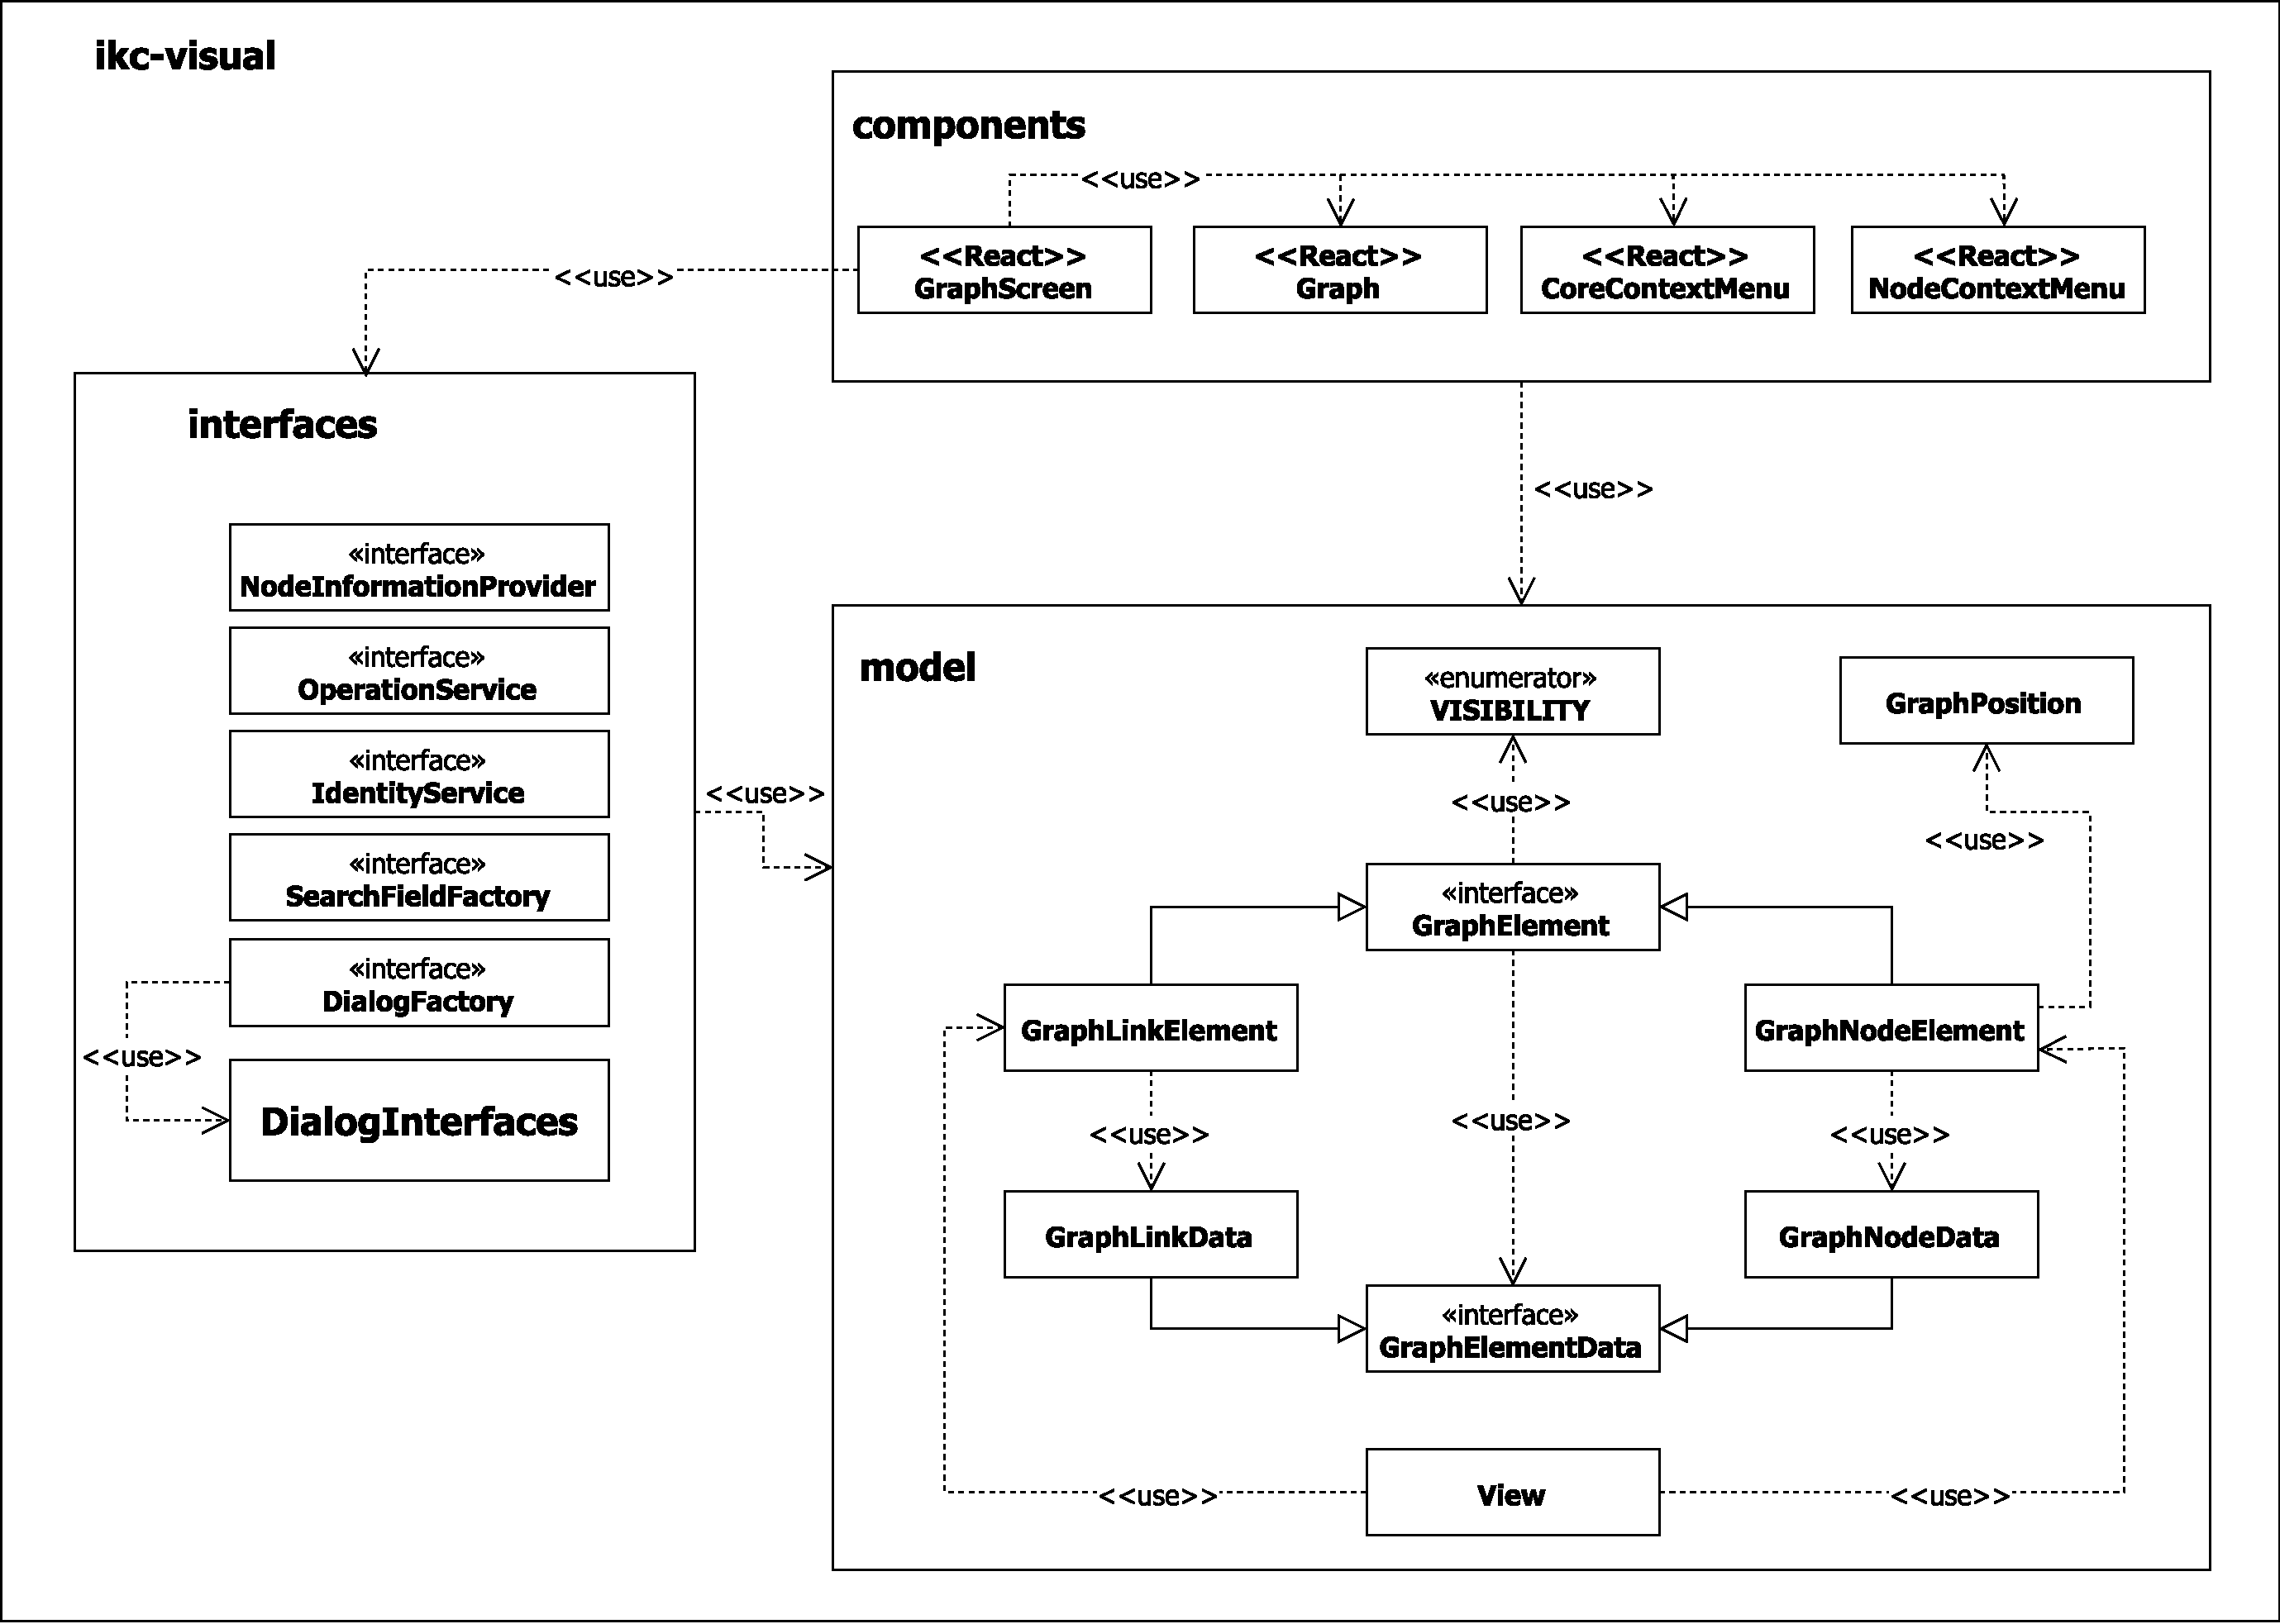
\includegraphics[width=1.6\textwidth]{architecture-overview}
\caption{Klassendiagramm}
\label{fig:klassendiagramm}
\end{figure}
\end{landscape}

\section{Schnittstellen} \label{schnittstellen}

Die hier gezeigten Schnittstellen dienen dem Austausch und der Interaktion mit dem \textit{ikc-core}. Um die Visualisierung in einer bestehenden Umgebung zu verwenden, müssen die erforderlichen Teile implementiert werden.

Die \autoref{fig:integration-ikc-core} zeigt einen Teil einer möglichen Integration, beispielsweise in den bestehenden \gls{ikc-core}. Die rechte Seite stellt einen Ausschnitt des \textit{ikc-visual}-Paketes an. Die Klasse \textit{GraphScreen} (\autoref{GraphScreenProps}) ist zu\-stä\-ndig für die Visualisierung des \gls{Netzwerk}[s]. Um den vollen Funktionsumfang zu bieten, benutzt sie, unter anderem, die Schnittstelle \textit{DialogFactory} (\autoref{DialogFactory}). Diese soll den Umgang mit Dialogfenstern ermöglichen. Da dies zu den grundlegenden Funktionen der Visualisierung zählt, befindet sich diese Schnittstelle direkt im \textit{ikc-visual}-Paket. Bei der Integration der Visualisierung in eine bestehende Umgebung gilt es somit, alle Schnittstellen entsprechend zu implementieren.

Die Klasse \textit{GraphVisualisation} verwendet die Klasse \textit{GraphScreen} aus der Visualisierung. Folglich muss beispielsweise die Schnittstelle \textit{DialogFactory} implementiert werden. Dies wird mit der Klasse \textit{GraphDialogFactory} realisiert.

Ähnlich wie beim oben beschriebenen Beispiel gibt es weitere Voraussetzungen des \textit{GraphScreen}, welche bei einer Integration beachtet werden sollten. Diese werden nachfolgend genau erläutert.

Es folgt eine Beschreibung der im \textit{ikc-visual}-Paket enthaltenen Klassen und Schnittstellen. 
\begin{figure}[htbp]
\centering
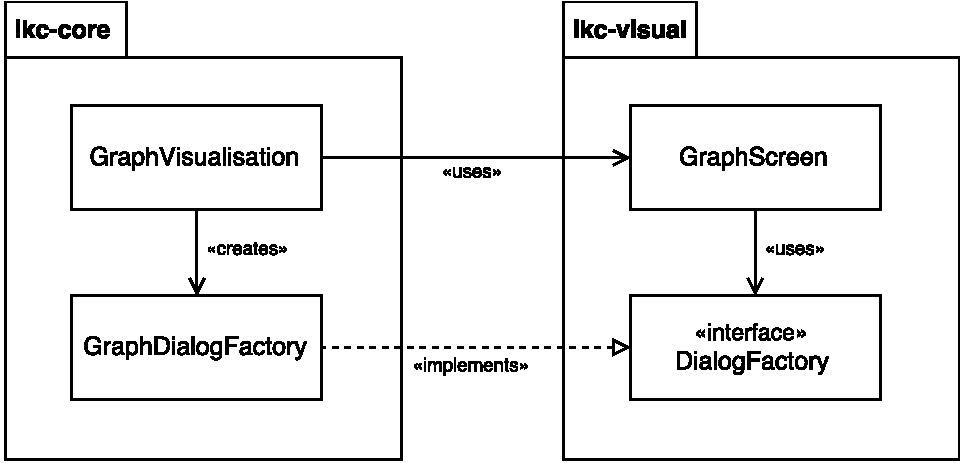
\includegraphics[width=0.7\textwidth]{architecture}
\caption{Integration \gls{ikc-core}}
\label{fig:integration-ikc-core}
\end{figure}

\subsection{GraphScreenProps}\label{GraphScreenProps}
Die \hyperref[react]{\textit{React}}-Komponente \textit{GraphScreen} wird seitens der Visualisierung implementiert. Sie ist die einzige, welche ausserhalb der Visualisierung genutzt werden kann. Damit ist deren Nutzung gleichzustellen mit der Nutzung der Visualisierung. Mit Hilfe der Schnittstelle \textit{GraphScreenProps} wird geregelt, wie die Komponente genutzt werden kann und welche Informationen, respektive welche Implementationen ihr zur Verfügung gestellt werden müssen.  

Somit sammelt die \textit{GraphScreen}-Komponente alle Abhängigkeiten und repräsentiert das \gls{Netzwerk} als Ganzes. Sie hält alle Referenzen zu Daten, Funktionen, sowie zu den umliegenden Komponenten. Damit stellt sie das einzige Bindeglied zwischen \gls{ikc-core} und der Visualisierung dar. Für die Verwendung der Komponente sind die folgenden Objekte bereitzustellen: Ein grosser Teil in Form von Implementationen von Schnittstellen, welche in der Visualisierung definiert sind. Diese werden in den nächsten Abschnitten genauer erläutert (\autoref{listing:graphscreen}):

\begin{itemize}
    \item \textit{viewToLoad} - View, welche angezeigt wird.
    \item \textit{nodeInformationProvider} - Stellt weitere Informationen zu \gls{Node}[s] und \gls{Link}[s] zur Verfügung.
    \item \textit{operationService} - Ermöglicht Interaktion mit der Datenbasis.
    \item \textit{timestamp} - Timestamp der letzten Verwendung.
    \item \textit{dialogFactory} - Ermöglicht den Zugriff auf die verschiedenen Dialoge.
    \item \textit{searchFieldFactory} - Ermöglicht den Zugriff auf die verschiedenen Suchfelder.
    \item \textit{onNodeDetailRequest} - \gls{Callback}-Methode, wenn weitere Informationen zu einem \gls{Node} gewünscht sind.
    \item \textit{nodeTypes} - Eine Liste verschiedener Arten von \gls{Node}[s], z.B. \textit{Plain}, \textit{Dropbox}, etc.
    \item \textit{identityService} - Ermöglicht das Erstellen von eindeutigen Indentifikationsnummern für neu erstellte \gls{Node}[s] und \gls{Link}[s]
\end{itemize}

\begin{listing}[htbp]
\inputminted[
frame=lines,
framesep=2mm,
baselinestretch=1.2,
linenos,
breaklines=true
]{js}{sourcecode/common/interfaces/GraphScreenProps.ts}
\caption{GraphScreen-Komponente}
\label{listing:graphscreen}
\end{listing}

In \autoref{listing:graphscreenexample} ist ein Beispiel für die Verwendung aufgezeigt. 

\begin{listing}[htbp]
\inputminted[
frame=lines,
framesep=2mm,
baselinestretch=1.2,
linenos,
breaklines=true
]{js}{sourcecode/GraphScreenExample.tsx}
\caption{GraphScreen-Beispiel}
\label{listing:graphscreenexample}
\end{listing}


\subsection{NodeInformationProvider}
\label{NodeInformationProvider}

Die Visualisierung benötigt für die Darstellung des \gls{Netzwerk}[s] diverse Informationen zu den einzelnen \gls{Node}[s] und \gls{Link}[s]. Dazu bietet der \textit{NodeInformationProvider} die beiden Methoden \texttt{getNodeTitle} und \texttt{getLinkLabel}. Die Identifikation erfolgt jeweils über eine eindeutige Identifikationsnummer (ID) (\autoref{listing:nodeinformationprovider}).

Teile der Visualisierung sollen mittels \gls{Drag'n'Drop} bedient werden können. Folgend ein Beispiel, wie die Schnittstelle in diesem Anwendungsfall benutzt werden kann:

Für ein \textit{Drag and Drop} wird üblicherweise ein \gls{Event} beim Loslassen des gepackten Elements ausgelöst. Das Element soll eine eindeutige ID enthalten. Dies ist aus dem bestehenden \textit{IKC-Core} vorausgesetzt. Wird das Element nun innerhalb der Visualisierung losgelassen, enthält der ausgelöste \gls{Event} diese ID. Sie wird zusammen mit dem \gls{Event} abgefangen und kann weiterverwendet werden. Beispielsweise können nun Informationen über den \textit{NodeInformationProvider} bezogen werden.

\begin{listing}[htbp]
\inputminted[
frame=lines,
framesep=2mm,
baselinestretch=1.2,
linenos,
breaklines=true
]{js}{sourcecode/common/interfaces/NodeInformationProvider.ts}
\caption{NodeInformationProvider-Interface}
\label{listing:nodeinformationprovider}
\end{listing}

Diese Schnittstelle deckt alle Leseoperationen ab. Schreiboperationen sind in der Schnittstelle \textit{OperationService} (\autoref{listing:operationservice}) zusammengefasst und werden im nächsten Abschnitt ausgeführt. 

\subsection{OperationService}
\label{OperationService}

Die \textit{OperationService}-Schnittstelle ermöglicht der Visualisierung Operationen an die Datenbasis weiterzuleiten. Damit spezifiziert und bün\-delt diese Schnittstelle alle Schreiboperationen, welche vom \gls{ikc-core} implementiert werden müssen (\autoref{listing:operationservice}). Diese Operationen entsprechen den folgenden vier Methoden:

\begin{enumerate}
  \item \texttt{createNodeFromDialogState} - neuer \gls{Node} auf der Basis des \textit{NewNode} Dialogs.
  \item \texttt{createNodeWithLinkFromDialogState} - neuer \gls{Node}, zusammen mit einem \gls{Link} zu einem bestehenden \gls{Node}, auf der Basis des \textit{NewNodeToConnect} Dialogs.
  \item \texttt{createLink} - neuer \gls{Link} definiert durch \textit{id}, den beiden \gls{Node}[s] \textit{source} und \textit{target} und dem entsprechenden \textit{label}.
  \item \texttt{saveView} - speichert die übergebene \gls{View}.
\end{enumerate}

\begin{listing}[htbp]
\inputminted[
frame=lines,
framesep=2mm,
baselinestretch=1.2,
linenos,
breaklines=true
]{js}{sourcecode/common/interfaces/OperationService.ts}
\caption{OperationService-Interface}
\label{listing:operationservice}
\end{listing}

\subsection{IdentityService}
\label{IdentityService}

Jeder \gls{Node} und jeder \gls{Link} in der Visualisierung als auch in der zugrundeliegenden Datenbasis verfügt über eine ID. Diese ermöglicht es, das Element eindeutig zu identifizieren und Operationen korrekt auszuführen. So kann ein konsistenter Kontext gewährleistet werden. Neue Elemente, welche aus der Visualisierung entstehen, müssen ebenfalls mit einer korrekten ID versehen werden. Dazu bietet die Schnittstelle \textit{IdentityService} (\autoref{listing:identityservice}) die beiden Methoden \texttt{create\-New\-Node\-Id} und \texttt{createNewLinkId}.

\begin{listing}[htbp]
\inputminted[
frame=lines,
framesep=2mm,
baselinestretch=1.2,
linenos,
breaklines=true
]{js}{sourcecode/common/interfaces/IdentityService.ts}
\caption{IdentityService-Interface}
\label{listing:identityservice}
\end{listing}

\subsection{DialogFactory}
\label{DialogFactory}
Durch die Entkopplung der Erstellung von Dialogen und der Visualisierung ist es möglich, die Visualisierung sehr flexibel einzusetzen. Die Visualisierung definiert zwar, welche Dialoge existieren, deren Implementation wird aber komplett ausgelagert. Diese Implementation ist für die Visualisierung nur soweit bedeutsam, als dass sie die benötigten Informationen liefert. Die Dialog-Schnittstellen definieren die dazu nötigen Eigenschaften. Diese Spezifikationen werden dann vom \gls{ikc-core} für die Implementation verwendet. Die verschiedenen Schnittstellen werden im nächsten \autoref{subsec:dialoginterfaces} detailliert behandelt.

%Mittels der Entkopplung, der Erstellung der nötigen Dialoge von der Visualisierung, wird ermöglicht die Visualisierung mit hoher Flexibilität zu verwenden. Die Visualisierung definiert welche Dialoge es gibt, wie diese jedoch konkret implementiert sind für die Visualisierung nicht bedeutsam solange diese die benötigen Informationen liefern. Dazu werden die Dialog Schnittstellen definiert und dadurch die zwingenden Eigenschaften der Dialoge. Diese Spezifikationen werden dann von dem \gls{ikc-core} für die Implementation verwendet. Die verschiedenen Schnittstellen werden im nächsten \autoref{subsec:dialoginterfaces} detailliert behandelt.\\
Mit Hilfe der Implementierung des \textit{DialogFactory}-Interfaces kann die Visualisierung die entsprechenden Dialoge erstellen und mit den nöt\-igen \gls{Callback} Methoden ausstatten. Dies funktioniert auch im Falle, dass die Implementation für die Visualisierung gänzlich unbekannt ist. Dabei handelt es sich um drei Dialoge, welche über separate Methoden adressiert werden können:

\begin{enumerate}
  \item \texttt{getDialogNodeNewNode} - liefert einen \textit{NewNode}-Dialog.
  \item \texttt{getDialogNodeNewNodeToConnect} - liefert einen \textit{New\-Node\-To\-Con\-nect}-Dialog.
  \item \texttt{getDialogNodeSearchToCon\-nect} - liefert einen \textit{Search\-Node\-To\-Con\-nect}-Dialog.
\end{enumerate}

\begin{listing}[htbp]
\inputminted[
frame=lines,
framesep=2mm,
baselinestretch=1.2,
linenos,
breaklines=true
]{js}{sourcecode/common/interfaces/DialogFactory.ts}
\caption{DialogFactory-Interface}
\label{listing:dialogfactory}
\end{listing}

\subsection{Dialog-Schnittstellen}
\label{subsec:dialoginterfaces}
Wie bereits aufgezeigt, übernehmen die Dialog Schnittstellen die Aufgabe, die minimalen Eigenschaften der verschiedenen Dialoge zu spezifizieren. Dies wird erreicht indem diese Schnittstellen als \textit{State}- und \textit{Props}-Interface verwendet werden.
%In den entsprechenden \hyperref[react]{\textit{React}} Implementierungen der Dialoge. 
Bei Bedarf können diese erweitert werden, um sie dem Kontext entsprechen anzupassen. Auf diese Weise wird erreicht, dass die Visualisierung die benötigten Informationen erhält. Diese Informationen nutzt sie danach, um die resultierenden Operationen der Dialoge auszuführen.

\subsubsection{NewNodeDialog}
Mittels des \textit{NewNode}-Dialogs wird es ermöglicht im \gls{ikc-core} einen Dialog zu nutzen, welcher dann seine Resultate direkt an die Visualisierung liefert. Die Schnittstelle \textit{DialogNewNodeProps} fungiert dabei als \textit{Props}-Interface. Mittels der Eigenschaft \texttt{type} wird der entsprechende Typ des zu erstellenden \gls{Node}[s] übergeben. Als Datencontainer (\texttt{node}) wird die Klasse \textit{GraphNodeElement} verwendet. Über die beiden \gls{Callback}-Methoden \texttt{on\-Request\-Close} und \texttt{onSave} wird die Visualisierung über die Endbedingungen des Dialogs informiert. In der Schnittstelle \texttt{DialogNewNodeState} wird der aktuelle Status des Dialogs gespeichert und schliesslich mit der Methode \texttt{onSave} an die Visualisierung übergeben. Dort kann der Status weiterverarbeitet werden.

\begin{listing}[htbp]
\inputminted[
frame=lines,
framesep=2mm,
baselinestretch=1.2,
linenos,
breaklines=true
]{js}{sourcecode/common/interfaces/DialogNewNodeInterfaces.ts}
\caption{DialogNewNode-Schnittstellen}
\label{listing:dialognewnode}
\end{listing}

\subsubsection{NewNodeToConnectDialog}
\label{NewNodeToConnectDialog}
Nebst der Erstellung eines \gls{Node}[s] soll es auch ermöglicht werden, mit Hilfe eines Dialogs einen neuen \gls{Node} zu erstellen, welcher mittels eines \gls{Link}[s] mit einem bestehenden \gls{Node} verbunden ist. Hierzu werden zwei zusätzliche Schnittstellen definiert: \textit{Dialog\-New\-Node\-To\-Con\-nect\-Props} und \textit{Dialog\-New\-Node\-To\-Con\-nect\-State}. Im Gegensatz zu den Schnittstellen des \textit{NewNodeDialog} wird hier als Datencontainer (\texttt{link}) für die Visualisierung die Klasse \textit{GraphLinkElement} verwendet.

\begin{listing}[htbp]
\inputminted[
frame=lines,
framesep=2mm,
baselinestretch=1.2,
linenos,
breaklines=true
]{js}{sourcecode/common/interfaces/DialogNewNodeToConnectInterfaces.ts}
\caption{DialogNewNodeToConnect-Interfaces}
\label{listing:dialognewnodetoconnect}
\end{listing}

\subsubsection{DialogNodeSearchToConnectInterfaces}
\label{DialogNodeSearchToConnectInterfaces}

Der dritte Dialog dient dazu, einen \gls{Node} aus der bestehenden Datenbasis zu suchen und diesen mit einem existierenden \gls{Node} in der Visualisierung mittels eines \gls{Link} zu verknüpfen. Wiederum werden die Eigenschaften dieses Dialogs mithilfe zweier Schnittstellen definiert: \textit{Dialog\-Node\-Search\-To\-Con\-nect\-Props} stellt wiederum sicher, dass die benötigten \gls{Callback}-Methoden zur Verfügung stehen. \textit{Dialog\-Node\-Search\-To\-Con\-nect\-State} sorgt dafür, dass die richtigen Informationen an die Visualisierung übergeben werden.

\begin{listing}[htbp]
\inputminted[
frame=lines,
framesep=2mm,
baselinestretch=1.2,
linenos,
breaklines=true
]{js}{sourcecode/common/interfaces/DialogNodeSearchToConnectInterfaces.ts}
\caption{DialogSearchNodeToConnect-Interfaces}
\label{listing:dialogsearchnodetoconnect}
\end{listing}


\subsection{SearchFieldFactory}
\label{SearchFieldFactory}
Sowohl das \textit{CoreContextMenu} als auch das \textit{NodeContextMenu} sind Komponenten, welche die Visualisierung liefert. Die integrierte Suche kann jedoch nicht von ihr zur Verfügung gestellt werden, da sie keinen Zugriff auf die zugrundeliegende Datenbasis hat%, insbesondere nicht auf die potentiell unterschiedlichen Suchalgorithmen
. Dazu wird die \textit{SearchFieldFactory} Schnittstelle verwendet, welche Zugriffe auf das \textit{NodeSearchField} und das \textit{LinkSearchField} regelt. Auch hier wird die konkrete Implementation der Suchkomponenten im \gls{ikc-core} erledigt.

Die einzelnen Komponenten werden über die Methoden \texttt{get\-Node\-Search\-Field} und \texttt{getLinkSearchField} geliefert. Dazu muss bei beiden eine \gls{Callback}-Methode übergeben werden, welche bei der Auswahl eines Suchresultats ausgeführt wird. Bei der Methode \texttt{get\-Link\-Search\-Field} muss zusätzlich ein \gls{Array} von den Link-IDs mitgeliefert werden. Darüber werden die Elemente festgelegt, welche bei der Suche berücksichtigt werden sollen.

\begin{listing}[htbp]
\inputminted[
frame=lines,
framesep=2mm,
baselinestretch=1.2,
linenos,
breaklines=true
]{js}{sourcecode/common/interfaces/SearchFieldFactory.ts}
\caption{SearchFieldFactory-Schnittstelle}
\label{lst:searchfieldfactory}
\end{listing}

\section{Model}\label{model}
Klassen oder Schnittstellen, welche sich auf die Haltung von Daten beschränken, %oder Enumeratoren 
werden als \textit{Model} zusammengefasst. So repräsentieren sie zum Beispiel eine Koordinate, einen Knoten oder einen Link. Da sie kein konkretes Verhalten implementieren, werden sie bereits im Lösungsdesign definiert. In anderen Sprachen, wie zum Beispiel \gls{Scala}, werden sie auch als sogenannte \textit{Case Classes} bezeichnet (\citep{caseClass}).

\subsubsection{GraphElement}
\label{GraphElement}
Die Schnittstelle \textit{GraphElement} ist das grundlegende Interface von \gls{Node}[s] und \gls{Link}[s]. Es wird durch zwei Eigenschaften spezifiziert (\autoref{lst:model-graphelement}):

\begin{itemize}
  \item \texttt{data} - enthält die nötigen Informationen zum jeweiligen Element. 
  %Die konkreten Klassen an dieser Stelle müssen die Schnittstelle \hyperref[GraphElementData]{\textit{GraphElementData}} implementieren um die Abstraktion dieser Schnittstelle sicherzustellen.
  \item \texttt{visibility} - beschreibt die Sichtbarkeit des Elements.
\end{itemize}

\begin{listing}[htbp]
\inputminted[
frame=lines,
framesep=2mm,
baselinestretch=1.2,
linenos,
breaklines=true
]{js}{sourcecode/common/model/GraphElement.ts}
\caption{GraphElement-Schnittstelle}
\label{lst:model-graphelement}
\end{listing}

\subsubsection{GraphElementData}
\label{GraphElementData}
Mit der einzigen Eigenschaft \texttt{id}, sorgt die Schnittstelle \textit{GraphElementData} für eine eindeutige Identifikation aller Elemente (\autoref{lst:model-graphelementdata}). 

\begin{listing}[htbp]
\inputminted[
frame=lines,
framesep=2mm,
baselinestretch=1.2,
linenos,
breaklines=true
]{js}{sourcecode/common/model/GraphElementData.ts}
\caption{GraphElementData-Interface}
\label{lst:model-graphelementdata}
\end{listing}

\subsubsection{GraphNodeElement}
\label{GraphNodeElement}
Die Klasse \textit{GraphNodeElement} repräsentiert einen einzelnen \gls{Node} und implementiert die Schnittstelle \hyperref[GraphElement]{\textit{GraphElement}}. Diese wird mit der Eigenschaft \texttt{position} erweitert, welche die aktuelle Position innerhalb der Visualisierung enthält und \texttt{nodeClasses}, um potentielle Node-Klassen zu speichern. Ebenfalls nutzt diese Klasse die entsprechende \hyperref[GraphElementData]{\textit{GraphElementData}} Implementierung \hyperref[GraphNodeData]{\textit{GraphNodeData}} . Ein \textit{GraphNodeElement} hat immer auch die gleiche ID und Titel wie in der Datenbasis, die restlichen Eigenschaften unterscheiden sich jedoch (\autoref{lst:model-graphnodeelement}).

\begin{listing}[htbp]
\inputminted[
frame=lines,
framesep=2mm,
baselinestretch=1.2,
linenos,
breaklines=true
]{js}{sourcecode/common/model/GraphNodeElement.ts}
\caption{GraphNodeElement-Klasse}
\label{lst:model-graphnodeelement}
\end{listing}

\subsubsection{GraphNodeData}
\label{GraphNodeData}
Die \gls{Node} spezifischen Daten werden in der Klasse \textit{GraphNodeData} gehalten. Diese entspricht einer konkreten Implementierung der Schnittstelle \hyperref[GraphElementData]{\textit{GraphElementData}}. Ergänzt wird sie durch die Eigenschaft \texttt{title}, welche den Titel des \gls{Node}[s] enthält (\autoref{lst:model-graphnodedata}).

\begin{listing}[htbp]
\inputminted[
frame=lines,
framesep=2mm,
baselinestretch=1.2,
linenos,
breaklines=true
]{js}{sourcecode/common/model/GraphNodeData.ts}
\caption{GraphNodeData-Klasse}
\label{lst:model-graphnodedata}
\end{listing}

\subsubsection{GraphLinkElement}
\label{GraphLinkElement}
Auch für die Repräsentation eines \gls{Link}[s] wird eine separate Implementation \textit{GraphLinkElement} der Schnittstelle \hyperref[GraphElement]{\textit{GraphElement}} verwendet. Mit der Eigenschaft \texttt{linkClasses} speichert sie eventuelle Link-Klassen. Auch hier wird zusätzlich eine Implementation \hyperref[GraphLinkData]{\textit{GraphLinkData}} der Schnittstelle \hyperref[GraphElementData]{\textit{GraphElementData}} für das \texttt{data} Objekt verwendet (\autoref{lst:model-graphlinkelement}).

\begin{listing}[htbp]
\inputminted[
frame=lines,
framesep=2mm,
baselinestretch=1.2,
linenos,
breaklines=true
]{js}{sourcecode/common/model/GraphLinkElement.ts}
\caption{GraphLinkElement-Klasse}
\label{lst:model-graphlinkelement}
\end{listing}

\subsubsection{GraphLinkData}
\label{GraphLinkData}
Auch für die \gls{Link} spezifischen Daten wird eine Implementation \textit{GraphLinkData} der Schnittstelle \hyperref[GraphElementData]{\textit{GraphElementData}} verwendet. Diese wird ergänzt durch die jeweiligen IDs \texttt{source} und \texttt{target} der \gls{Node}[s], welche den \gls{Link} mit den jeweiligen \gls{Node}[s] verbindet und ein entsprechendes Label (\texttt{label}) (\autoref{lst:model-graphlinkdata}).

\begin{listing}[htbp]
\inputminted[
frame=lines,
framesep=2mm,
baselinestretch=1.2,
linenos,
breaklines=true
]{js}{sourcecode/common/model/GraphLinkData.ts}
\caption{GraphLinkData-Klasse}
\label{lst:model-graphlinkdata}
\end{listing}

\subsubsection{GraphPosition}
Um eine Position in der Visualisierung zu persistieren, werden die X- und Y-Koordinaten gespeichert. Dazu wird die Klasse \textit{GraphPosition} verwendet (\autoref{lst:model-graphposition}). 

\begin{listing}[htbp]
\inputminted[
frame=lines,
framesep=2mm,
baselinestretch=1.2,
linenos,
breaklines=true
]{js}{sourcecode/common/model/GraphPosition.ts}
\caption{GraphPosition-Klasse}
\label{lst:model-graphposition}
\end{listing}

\subsubsection{View}\label{view}
Um die verschiedenen \gls{View}s und die Positionen der enthaltenen \gls{Node}[s] zu persistieren, wird die Klasse \gls{View} verwendet. Sie enthält dabei die grundlegende Struktur des gesamten \gls{Netzwerk}[s]. Mit Hilfe des Enumerators VISIBILITY (\autoref{VISIBILITY}) wird festgelegt, welche \gls{Link}[s] und \gls{Node}[s] tatsächlich auch dargestellt werden. Dazu hat sie die folgenden Eigenschaften: (\autoref{lst:model-view}):

\begin{itemize}
  \item \texttt{id} - eindeutige Identifikation.
  \item \texttt{titel} - Titel des \gls{Node}[s].
  \item \texttt{changedAt} - Timestamp der letzten Aktualisierung.
  \item \texttt{createdAt} - Timestamp der Erstellung.
  \item \texttt{nodes} - Liste aller \gls{Node}[s] der Datenbasis. In der Visualisierung werden die einzelnen \gls{Node}[s] abhängig von der Eigenschaft \texttt{vi\-si\-bi\-li\-ty} dargestellt.
  \item \texttt{links} - Liste aller \gls{Link}[s] der Datenbasis. Auch hier werden die \gls{Link}[s] anhand der Eigenschaft \texttt{visibility} dargestellt oder nicht.
\end{itemize}

\begin{listing}[htbp]
\inputminted[
frame=lines,
framesep=2mm,
baselinestretch=1.2,
linenos,
breaklines=true
]{js}{sourcecode/common/model/View.ts}
\caption{View-Klasse}
\label{lst:model-view}
\end{listing}

\subsubsection{VISIBILITY}\label{VISIBILITY}
Mit dem Enumerator \textit{VISIBILITY} wird die Sichtbarkeit eines Elements festgelegt. Die ist entweder \texttt{VISIBLE} oder \texttt{HIDDEN} (\autoref{lst:model-view}). Da \hyperref[typescript]{\textit{Typescript}} keine String-Enumeratoren kennt, wird stattdessen eine normale Klasse verwendet.

\begin{listing}[htbp]
\inputminted[
frame=lines,
framesep=2mm,
baselinestretch=1.2,
linenos,
breaklines=true
]{js}{sourcecode/common/model/VISIBILITY.ts}
\caption{VISIBILITY-Enumerator}
\label{lst:model-enumerator}
\end{listing}


\section{Framework-Auswahl}
Um sicherzustellen, dass ein geeignetes \gls{Framework} für die Visualisierung verwendet wird, müssen verschiedene Optionen untersucht und bewertet werden.

\subsection{Kriterien-Katalog}
Für die Bewertung wird ein Katalog an Kriterien definiert, welcher sich an den definierten Anforderungen (siehe \autoref{anforderungen}), der Risikoanalyse (siehe \autoref{risikoanalyse}), den Schnittstellen (siehe \autoref{schnittstellen}) und den Komponenten (siehe \autoref{komponenten}) orientiert. Folgend eine Übersicht über den Kriterienkatalog (\autoref{tab:kriterien-katalog}). 

\begin{longtable}{|p{1cm}| P{3cm} | P{8.1cm}|}
  \hline
    ID & Titel & Beschreibung \\\hline
    K1 & Mobile Darstellung & Das \gls{Framework} kann im mobilen Umfeld verwendet werde\\\hline
    K2 & Operationen & Es können die folgenden Operationen umgesetzt werden:
        \begin{enumerate}
          \item Einen neuen \gls{Node} innerhalb der Visualisierung erstellen.
          \item Zwei \gls{Node}[s] innerhalb der Visualisierung verbinden.
          \item Einen \gls{Node} innerhalb der Visualisierung löschen.
        \end{enumerate} \\\hline
    K3 & Operationen (D'n'D\footnote{Drag and Drop.}) & Es können die folgenden D'n'D-Operationen umgesetzt werden:
        \begin{enumerate}
          \item Einen neuen \gls{Node} mittels \gls{Drag'n'Drop} innerhalb der Visualisierung erstellen.
          \item Zwei \gls{Node}[s] innerhalb der Visualisierung mittels \gls{Drag'n'Drop} verbinden.
        \end{enumerate} \\\hline
    K4 & \gls{Node} Details & \gls{Node} Details können angezeigt und bearbeitet werden.\\\hline
    K5 & Menü & Ein Kontextmenü für weitere Operationen anzeigen.\\\hline
    K6 & \gls{Node}[s] Speichern & Positionen der \gls{Node}[s] können gespeichert werden.\\\hline
    K7 & \gls{Node}[s] Laden & Eine bestehende View kann dargestellt werden.\\\hline
    K8 & \gls{Toolbox} & Weitere Operationen, z.B. eine Suche, können in einer \gls{Toolbox} angeboten werden.\\\hline
    K9 & Komplexität & Allgemeiner Eindruck des \gls{Framework}s hinsichtlich der Komplexität.\\\hline
    K10 & Erweiterbarkeit & Allgemeiner Eindruck des \gls{Framework}s hinsichtlich der Erweiterbarkeit.\\\hline
    K11 & Dokumentation & Das \gls{Framework} ist gut dokumentiert, es gibt genügend Beispiele und eine entsprechende \textit{Community} zur allfälligen Unterstützung.\\\hline
    \caption{Kriterienkatalog}
  \label{tab:kriterien-katalog}
\end{longtable}
Mit Hilfe dieses Katalogs sollen die Möglichkeiten, Chancen und auch Risiken der verschiedenen \gls{Framework}s identifiziert werden. Aufgrund dieses Prozesses kann anschliessend eine genaue Einschätzung der Möglichkeiten und des Aufwands aufgestellt werden. Die verschiedenen \gls{Framework}s werden anhand der folgenden Skala bewertet (1-5): 
\begin{enumerate}
  \item Die Erfüllung des Kriteriums \textbf{ohne} Anpassungen möglich.
  \item Die Erfüllung des Kriteriums mit \textbf{leichten} Anpassungen möglich.
  \item Die Erfüllung des Kriteriums ist \textbf{mit Anpassungen} möglich.
  \item Die Erfüllung des Kriteriums ist mit \textbf{grossen} Anpassungen mög\-lich.
  \item Die Erfüllung des Kriteriums ist \textbf{nicht} möglich.
\end{enumerate}

\subsection{Ergebnisse}
Aufgrund des definierten Kriterienkataloges wurden die verschiedenen \gls{Framework}s untersucht und bewertet. Die Ergebnisse sind in der folgenden \autoref{tab:framework-auswertung} aufgeführt. Die Tabelle widerspiegelt die Eindrücke und Erfahrungen, welche während den Untersuchungen gemacht wurden:

Zwar sind auch die umfassenderen Lösungen sehr interessant, jedoch ist deren Verwendung für den hier notwendigen Zweck zu kompliziert. Es würde lediglich ein kleiner Teilbereich der bereits bestehenden Lösung genutzt. Um aber diesen erfolgreich einzusetzen, ist dennoch tiefe Kenntnis des jeweiligen \gls{Framework}s erforderlich. Dies sprengt schlichtweg den zeitlichen Rahmen und ist auch nicht notwendig. Die nötigen Erweiterungen können in den anderen, schlankeren \gls{Framework}s ohne grossen Zusatzaufwand ergänzt werden.

Darum fiel die Wahl eindeutig auf \textit{cytoscape.js}. Es beschränkt sich lediglich auf die Darstellung von \gls{Netzwerk}[en]. Diverse Erweiterungen sind bereits zugänglich. Zudem ist es gleichzeitig relativ einfach den Funktionsumfang eigenhändig zu ergänzen.

\begin{longtable}{|p{0.8cm}| p{2.2cm} | p{1.5cm}| p{1.5cm}| p{2cm}| p{2cm}|}
  \hline
    & \textit{cytoscape.js} & \textit{greuler} &\textit{JointJS} &\textit{jsPlumb} &\textit{mxGraph}  \\\hline
    Total & 23 & 27 & 38 & 24 & 27\\\hline
    \caption{Framework-Auswerung}
  \label{tab:framework-auswertung}
\end{longtable}

\subsection{Bewertungen}\label{Bewertungen}
Eine detaillierte Bewertung der fünf verschiedenen \gls{Framework}s kann den folgenden Abschnitten entnommen werden.

\subsubsection{cytoscape.js}
\label{cytoscape}
Cytoscape ist eine \textit{open-source} Javascript Bibliothek für Graphen- oder \gls{Netzwerk}-Theorie. Sie eignet sich nicht nur für Visualisierungen, sondern auch für Analysen. Cytoscape ist mit allen gängigen Browsern und Bibliotheken kompatibel. Zudem funktioniert die Darstellung ohne zusätzlichen Aufwand auf allen Bildschirmgrössen. Es gibt zahlreiche Erweiterungen und auch die Integration in bestehende Lösungen ist einfach möglich. \citep{1_franz_lopes_huck_dong_sumer_bader_2016}

Wie in \autoref{fig:bsp-cytoscape} ersichtlich, beschränkt sich die Bibliothek auf die Visualisierung von \gls{Netzwerk}[en]. Standardmässig sind keine Zusatzfunktionen, beispielsweise das Interagieren mit \gls{Node}[s] und \gls{Link}[s] möglich. Die Bibliothek ist sehr schlank gehalten, was eine einfache Integration und Erweiterung stark vereinfacht. Das \gls{Netzwerk} wird direkt im \textit{JSON}-Format hinterlegt. Bei Änderungen werden die hinterlegten Daten angepasst und anschliessend angezeigt.

\begin{figure}[htbp]
\centering
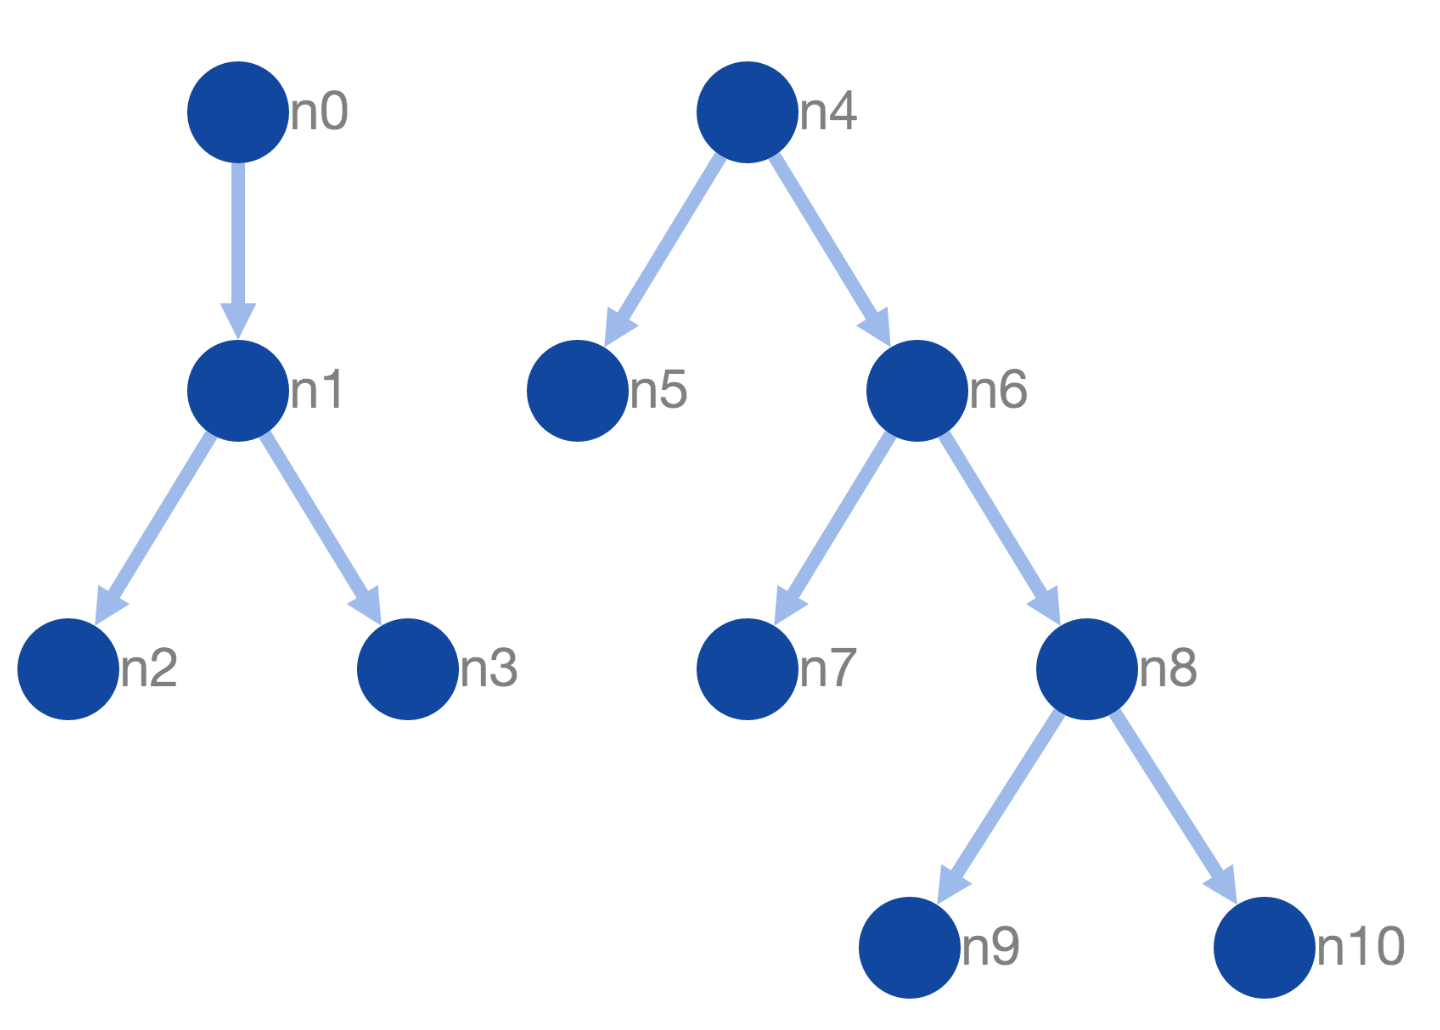
\includegraphics[width=0.4\textwidth]{cytoscape}
\caption{Beispiel Cytoscape}
\label{fig:bsp-cytoscape}
\end{figure}


\begin{longtable}{|p{0.5cm}|p{0.5cm}|p{0.5cm}|p{0.5cm}|p{0.5cm}|p{0.5cm}|p{0.5cm}|p{0.5cm}|p{0.5cm}|p{0.7cm}|p{0.7cm}|}
  \hline
    K1 & K2 & K3 & K4 & K5 & K6 & K7 & K8 & K9 & K10 & K11 \\\hline
    2 & 2 & 2 & 2 & 2 & 2 & 3 & 2 & 2 & 3 & 1\\\hline
    \caption{Bewertung  \textit{cytoscape.js}}
  \label{tab:bewertung-cytoscape}
\end{longtable}

\subsubsection{greuler}
Hier gibt es viele Parallelen zur vorgängigen Bibliothek (\textit{cytoscape.js}). \textit{Greuler} spezialisiert sich nun aber auf die Visualisierung und baut wie viele andere auf \textit{D3}. Bezüglich der Handhabung ist es grösstenteils identisch mit \textit{Cytoscape}, allerdings hat es hier bei weiten nicht so viele Erweiterungsmöglichkeiten. \autoref{fig:bsp-greuler} zeigt ein kleines Beispielnetzwerk. \citep{2_maurizzzio/greuler_2016}

\begin{figure}[htbp]
\centering
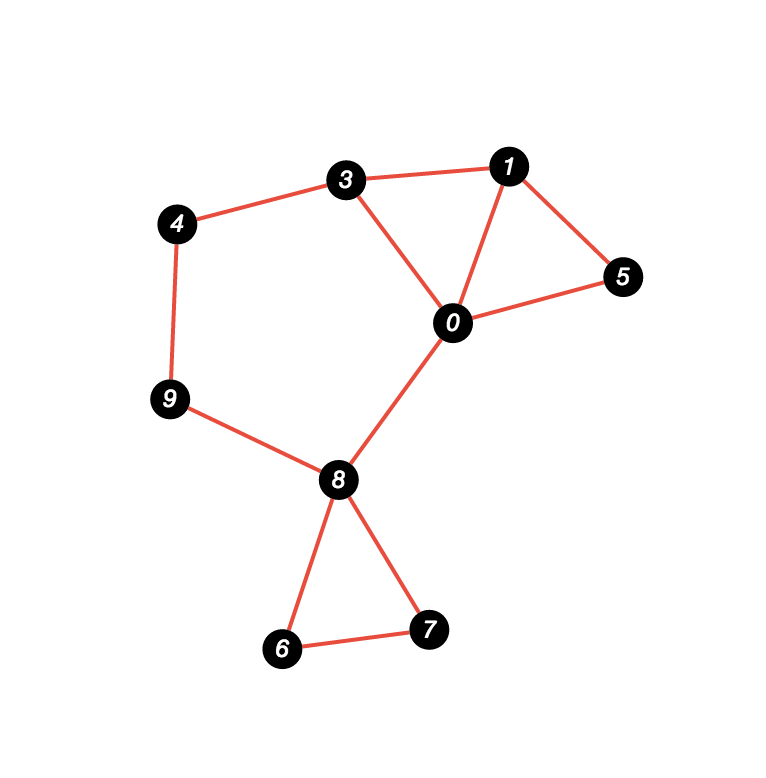
\includegraphics[width=0.4\textwidth]{greuler}
\caption{Beispiel Greuler}
\label{fig:bsp-greuler}
\end{figure}

\begin{longtable}{|p{0.5cm}|p{0.5cm}|p{0.5cm}|p{0.5cm}|p{0.5cm}|p{0.5cm}|p{0.5cm}|p{0.5cm}|p{0.5cm}|p{0.7cm}|p{0.7cm}|}
  \hline
    K1 & K2 & K3 & K4 & K5 & K6 & K7 & K8 & K9 & K10 & K11 \\\hline
    2 & 2 & 2 & 2 & 2 & 4 & 4 & 2 & 2 & 4 & 3\\\hline
    \caption{Bewertung \textit{greuler}}
  \label{tab:bewertung-greuler}
\end{longtable}

\subsubsection{JointJS}
Auch bei JointsJS handelt es sich um eine \textit{open-source}-Bibliothek. Im Gegensatz zu den obigen beiden geht die Funktionalität eine Ebene weiter. Hier werden zusätzlich zur eigentlichen Darstellung auch Werkzeuge zur Manipulation des Diagramms mitgeliefert. Viele Funktionalitäten sind aber erst mit der kostenpflichten Version \textit{Rappid} ver\-füg\-bar, welche auf JointJS aufbaut. \citep{jointsjs}

Die Bibliothek ist für den hier vorliegenden Anwendungsfall zu umfangreich. Die vielen Funktionen machen die Implementation sehr komplex. Dieser Aufwand ist für die eigentlich einfache Anwendung zu gross. Die Vorteile, welche der vorhandene Funktionsumfang bietet, erkennt man erst nach längerer Einarbeitung. Der notwendige Funktionsumfang kann in anderem \gls{Framework}[s] ohne grossen Aufwand selbst implementiert werden. So ist die Übersicht stets geboten und der Code bleibt verhältnismässig einfach.

\begin{longtable}{|p{0.5cm}|p{0.5cm}|p{0.5cm}|p{0.5cm}|p{0.5cm}|p{0.5cm}|p{0.5cm}|p{0.5cm}|p{0.5cm}|p{0.7cm}|p{0.7cm}|}
  \hline
    K1 & K2 & K3 & K4 & K5 & K6 & K7 & K8 & K9 & K10 & K11 \\\hline
    1 & 3 & 3 & 3 & 3 & 4 & 4 & 5 & 4 & 5 & 3\\\hline
    \caption{Bewertung \textit{JointJS}}
  \label{tab:bewertung-jointjs}
\end{longtable}

\subsubsection{jsPlumb}
\label{jsPlumb}

\begin{longtable}{|p{0.5cm}|p{0.5cm}|p{0.5cm}|p{0.5cm}|p{0.5cm}|p{0.5cm}|p{0.5cm}|p{0.5cm}|p{0.5cm}|p{0.7cm}|p{0.7cm}|}
  \hline
    K1 & K2 & K3 & K4 & K5 & K6 & K7 & K8 & K9 & K10 & K11 \\\hline
    2 & 2 & 2 & 1 & 3 & 2 & 2 & 2 & 3 & 3 & 2\\\hline
    \caption{Bewertung \textit{jsPlumb}}
  \label{tab:bewertung-jsplumb}
\end{longtable}

Als einzige Bibliothek basiert jsPlump auf reinen \gls{HTML}-Objekten. Somit werden diese nicht in einem \gls{Canvas} gezeichnet, sondern wie normaler \gls{HTML} Code dargestellt. Somit kann das Aussehen der Elemente direkt durch \gls{CSS}-Klassen angepasst werden. 

\clearpage

Jedoch legt jsPlump den Fokus vor allem auf das Zeichnen und Erstellen von Diagrammen. Es bietet daher eine grosse Anzahl von Funktionen, welche nicht benötigt werden. Zusätzlich müssten benötigte Funktionen zum Teil manuell implementiert werden. Ebenfalls ist nur die limitierte \textit{Community Edition} kostenlos verfügbar. \citep{jsplump}

\begin{figure}
\centering
\begin{subfigure}[b]{0.5\textwidth}
   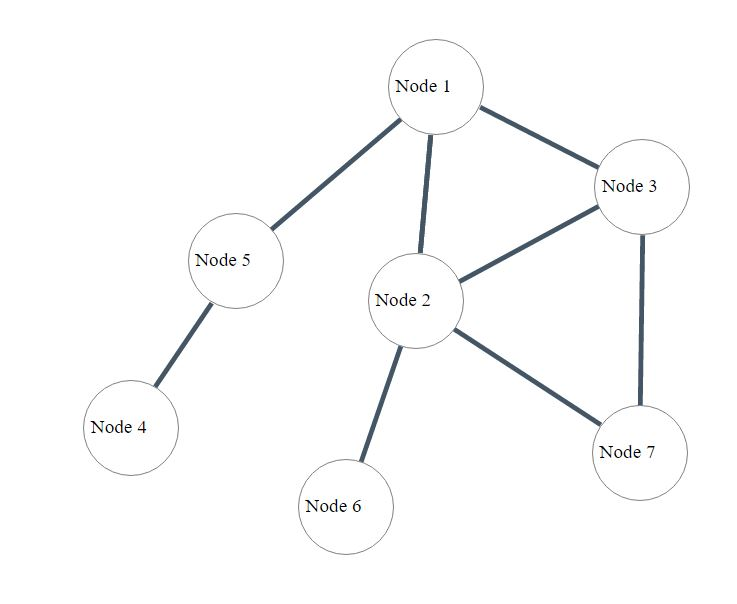
\includegraphics[width=0.9\linewidth]{JsPlump}
\caption{Beispiel JsPlump}
\label{fig:bsp-jsplump}
    \end{subfigure}
\begin{subfigure}[b]{0.4\textwidth}
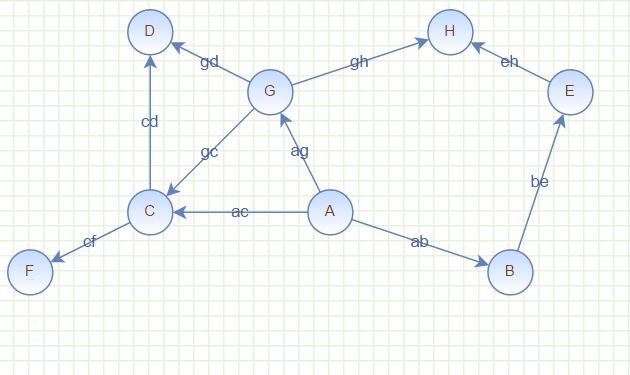
\includegraphics[width=0.9\linewidth]{MxGraphEval}
\caption{Beispiel mxGraph}
\label{fig:bsp-mxgraph}
    \end{subfigure}
    \caption{Frameworks}
\end{figure}



\subsubsection{mxGraph}
Wie auch schon bei der Bibliothek jsPlump setzt mxGraph den Fokus auf die Darstellung und Bearbeitung von ganzen Diagrammen. Es wurde schon als Grundlage von grossen Anwendung wie \textit{draw.io} verwendet. Dadurch ist eine Vielzahl von Funktionen verfügbar. Jedoch würde sich eine Erweiterung dieser eher kompliziert gestalten. \citep{mxGraph}

\begin{longtable}{|p{0.5cm}|p{0.5cm}|p{0.5cm}|p{0.5cm}|p{0.5cm}|p{0.5cm}|p{0.5cm}|p{0.5cm}|p{0.5cm}|p{0.7cm}|p{0.7cm}|}
  \hline
    K1 & K2 & K3 & K4 & K5 & K6 & K7 & K8 & K9 & K10 & K11 \\\hline
    2 & 3 & 3 & 2 & 3 & 2 & 2 & 2 & 4 & 4 & 2\\\hline
    \caption{Bewertung \textit{mxGraph}}
  \label{tab:bewertung-mxgraph}
\end{longtable}
